
% The subsections written are only suggestions to display how sections and subsections may look for your thesis

\section{Motivation}
Contemplative practices, traditional methods of disciplined mental and physical training, enhance self-awareness, inquiry, and regulation \cite{Davidson2017VarietiesOC}. They promote sustained, non-judgmental attention and introspection, providing a peaceful refuge in daily life. This centered tranquility aids in exploring life's deeper meanings and values. Among these practices are meditation, yoga, breathwork, prayer, and mindful walking \cite{Bruce2018ContemplativePP}. \footnote{The motivation for this master thesis is based on the motivation from the preceding project thesis on the same topic provided in \autoref{Appendix C}}

Traditionally maintained by spiritual figures like priests and yogis, these practices have recently gained broader popularity \cite{Brandmeyer2021MeditationAT}. Recent studies have found that 14.3\% of U.S. adults practice yoga and meditation, with about 17.5\% engaging in some form of mind-body therapy \cite{14USA}\cite{33USA}. During the COVID-19 pandemic's initial wave in Norway, nearly a quarter of the population turned to self-help practices such as yoga and meditation \cite{Norge}. The appeal of mindfulness practices is linked to their numerous benefits, including mental and physical health improvements and cognitive enhancements in various age groups \cite{happyreinforcment}\cite{agecognition}.

The increased public interest in these practices has spurred a wave of scientific studies \cite{Brandmeyer2021MeditationAT}. Research has predominantly explored how these practices alter brain structure and function, thereby improving behavioral, medical, and professional outcomes \cite{Brandmeyer2021MeditationAT}. Techniques like Mindfulness-Based Stress Reduction (MBSR) and yogic breathing have been shown to reduce symptoms of anxiety, depression, and PTSD \cite{metamindfullnes}\cite{yogabreathing}. However, the field is characterized by methodological inconsistencies and small sample sizes, complicating the drawing of broad conclusions \cite{metamindfullnes}.

Studies often depend on self-reported measures to assess outcomes, as noted by \cite{deconReconSelf}:

\begin{quote}
"Though preliminary findings suggest that meditation and other forms of mental training may produce demonstrable changes in subjective experience, behavior, patterns of neural activity, and peripheral biology, rigorous studies are still needed to uncover the precise mechanisms that underlie these changes. In particular, randomized trials, active control groups, longitudinal studies that examine within- and across-subject changes over time, and across-practice comparisons will be significant in determining the efficacy of meditation training paradigms."
\end{quote}

However, integrating objective physiological markers, such as neural activity or hormone levels, could provide a more comprehensive understanding of these practices' mechanisms. Combined with self-reported and behavioral measures, triangulation of the underlying state could yield a more complete picture. \cite{SmallwoodSchooler2015}\cite{Schooler2004}

A recent study comparing the practices of Cyclic Sighing and Mindfulness Meditation reported that Cyclic Sighing significantly enhanced mood and relaxation when practiced daily for five minutes, suggesting immediate benefits over Mindfulness Meditation for mood improvement and stress reduction \cite{huberman2022contemplative}.

While the primary objective of mindfulness practices is to develop a quality of present-moment focus, characterized by curiosity, openness, and acceptance \cite{deconReconSelf}, the study of these practices fundamentally revolves around the study of attention.

Historical research posits that effort equates to attention, linked to sympathetic dominance in the autonomic nervous system and increased metabolic brain activity \cite{Kahneman1973AttentionAE}. However, recent findings suggest that attention can also occur under parasympathetic dominance, experienced as effortless \cite{Tang2019PromotingPW}\cite{BruyaTang2018}. Thus, two types of attention exist: one tied to sympathetic dominance (e.g., control, tonic alertness) and another associated with parasympathetic dominance (e.g., monitoring, phasic alertness) \cite{posner2015}\cite{posner2020_2022}.

Different neural pathways are engaged in effortful and effortless training \cite{posner2020_2022}. Effortful training activates the frontoparietal brain regions and is linked to sympathetic dominance. In contrast, effortless training involves the anterior cingulate cortex (ACC), posterior cingulate cortex (PCC), and striatum, fostering parasympathetic responses like reduced heart rate and increased high-frequency heart rate variability (HF-HRV), which are beneficial in various medical conditions \cite{singer2016training}\cite{HRV}.

Measures such as Electrocardiogram (ECG), which can assess HRV, help categorize contemplative practices based on their sympathetic and parasympathetic responses. However, the assumption that low-frequency (LF) HRV is indicative of sympathetic control has been challenged, suggesting that additional measures like Electroencephalogram (EEG) are necessary for conclusive classifications \cite{reyes2013utility}\cite{valenza2016disentanglement}.

A more mature field of study related to contemplative practices is the study of mind wandering. In mind-wandering research, an important split is between the perceptually generated and the self-generated experience, as well as on-task or off-task (task-unrelated) behavior. Whereas on-off task behavior relates to a set goal, the perceptual-self-generation split refers to the split between stimuli from the inside and the outside world. Hence, we get a 2x2 matrix of possible classifications described in \autoref{fig: mw_split} taken from \cite{SmallwoodSchooler2015}. 
%\begin{comment}
\begin{figure}[H]
    \centering
    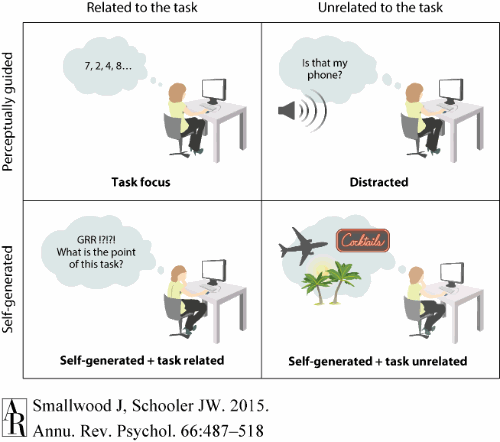
\includegraphics[width=300px]{Figures/mw_split.png}
    \caption{Perceptually vs. Self-generated and on-off task split taken from \cite{SmallwoodSchooler2015}.}
    \label{fig: mw_split}
\end{figure}
%\end{comment}

Here, off-task self-generated thought is called mind-wandering, the opposite of mindful attention. Several studies have examined mind-wandering imprint on EEG data\cite{Kam2011}. A few publicly available datasets can also be found \cite{Jin2019PredictingMW}\cite{DelormeEEGMeditationStudy}\cite{Rodriguez-Larios2020}\cite{DelormeEGGMeditationThinking}. Hence, by building on the mind-wandering literature, a device for the estimation of meditative proficiency and progress can be built.



%\section{Project description}

%This master's thesis continues the project thesis written in fall 2023 in \autoref{Appendix B}. The thesis aims to lay a foundation for studying contemplative practices using lab-grade objective measurement tools focusing on EEG and building a classification tool for estimating contemplative proficiency and progress. The thesis's main contribution to this goal is a code base for a Convolutional Neural Network classification tool built upon the EEGNeX architecture and preliminary data analysis of the study conducted in the project thesis.

\section{Scope of the Overall Project}

The primary objective of the Contemplative Neuroscience Project is to develop a method for more accurately measuring the meditation progress of novice meditators. This necessitates integrating subjective and objective measurements to provide a more comprehensive estimate of progress than either approach could achieve independently. Reliable estimates of meditation progress could be instrumental in subsequent studies to identify the most effective techniques for learning meditation. On a personal level, these estimates could offer novice meditators more precise guidance, potentially reducing dropout rates.

This knowledge is crucial for selecting specific practices to achieve desired health and wellness outcomes, which may enhance quality of life and benefits in healthcare and personal development. For example, practices that elicit parasympathetic responses, such as reduced heart rate and increased heart rate variability, can be strategically employed for relaxation, cardiovascular health, and cognitive enhancement. High-quality progress assessments could thus have practical implications for managing the stressors of modern life and addressing mental health challenges. This potential aligns with the development goals outlined in the United Nations Sustainable Development Goal 3, which aims to ensure healthy lives and promote well-being for all ages (\cite{UN_SDG3_2023}).

\begin{figure}[h!]
    \centering
    
\includegraphics[width=0.3\linewidth]{Figures/goal3.jpg}
    \caption{UN Sustainable Development Goal 3: Ensure healthy lives and promote well-being at all ages.}
    \label{fig:goal3}
\end{figure}

Several pieces need to come together to achieve this long-term goal, as shown in \autoref{fig:overal_goal}.
The first step involves gathering EEG data from novice meditators during meditation sessions. This data will be the foundation for developing and refining objective analysis tools. Regular sessions should be recorded to capture meditative experiences and mind-wandering episodes.

By utilizing the collected data, the next step is to design and build machine learning models—specifically, classification tools capable of distinguishing between states of mind wandering and focused attention. This involves training Convolutional Neural Networks (CNNs) or other suitable algorithms on the EEG data to classify the cognitive states accurately.

With the classification tools, each meditator's progression can be tracked over time. By analyzing the trends in the classification data, insights into how an individual's ability to maintain focused attention or control mind wandering evolves with practice can be drawn. This longitudinal analysis is crucial for assessing the effectiveness of the meditation practice.

To enhance the robustness of the findings, the objective data obtained from the EEG analysis should be integrated with subjective data collected through questionnaires in a triangulation format. These questionnaires can gather personal insights from the meditators about their experiences, challenges, and perceived progress, providing a comprehensive view of their meditation journey.

Finally, the comprehensive data analysis setup will be leveraged to guide individual meditators and facilitate progress analysis. Based on the trends observed in their data, specific recommendations can be made to help them optimize their practice, overcome challenges, and achieve better mental health outcomes.

\begin{figure}[H]
    \centering
    \hspace*{-2cm} 
    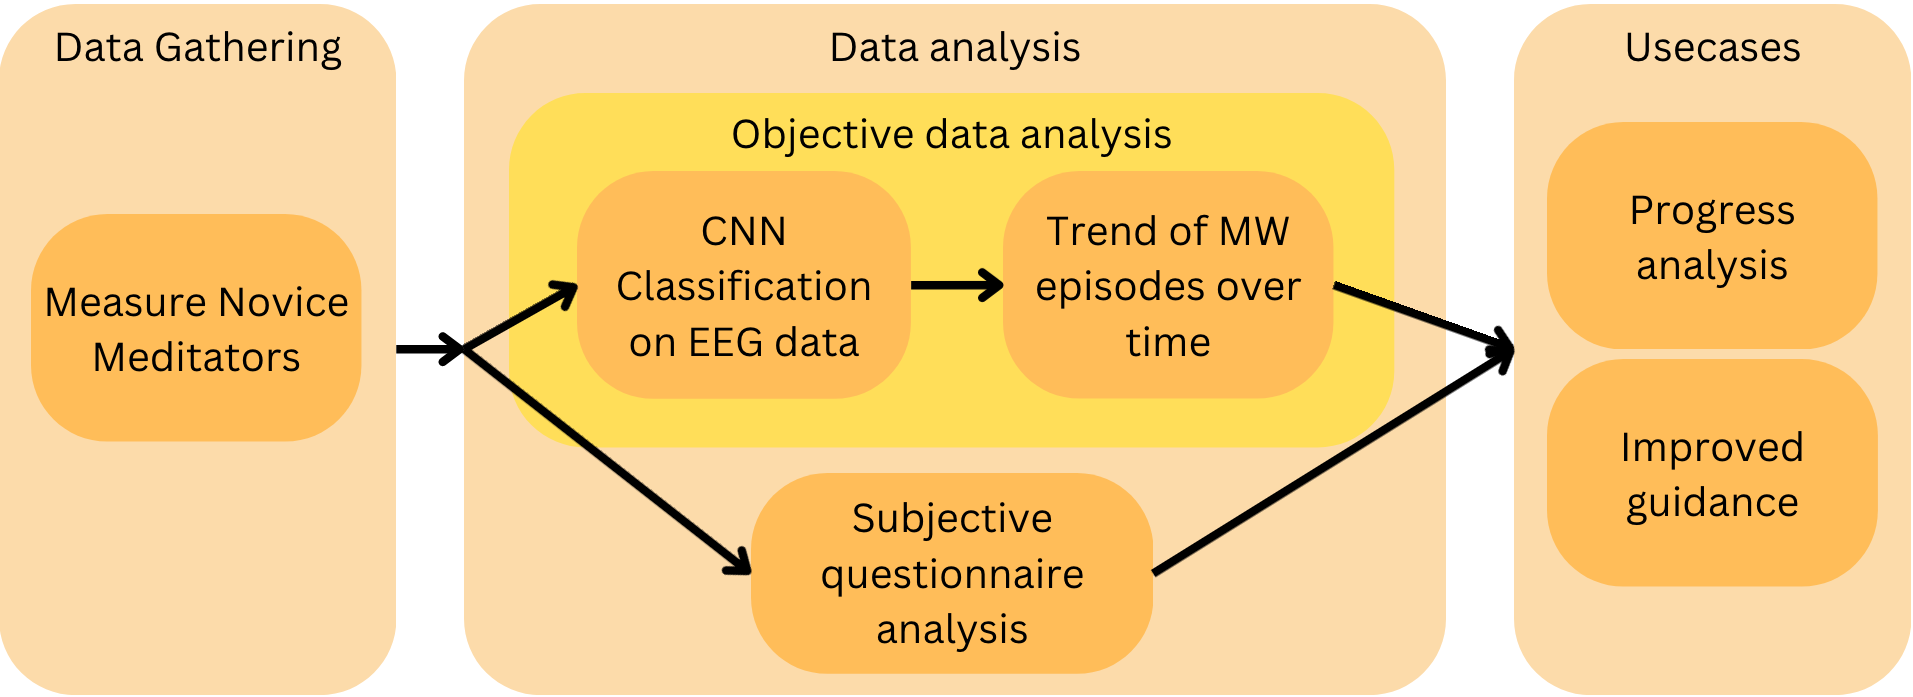
\includegraphics[width=500px]{Figures/project_flow.png}
    \caption{Overall project Goal.}
    \label{fig:overal_goal}
\end{figure}

Zooming in on the CNN classification from \autoref{fig:overal_goal}, several parts need to be implemented for the best estimates of Mind Wandering as shown in \autoref{fig:cnn_goal}. The training data for CNN can come from online datasets or be developed internally to secure high-quality data. Then, it's the CNN implementation, finding the best underlying architectures, model designs, and design choices for what parameters to include. Optimization is another significant step in parameter optimization and selecting the best channels. This could reduce time as some channels are likely more important for prediction while others give less valuable information. At last, the CNN needs to be validated on another dataset to see that it performs well on unseen data and is reliable. 

\begin{figure}[H]
    \centering
    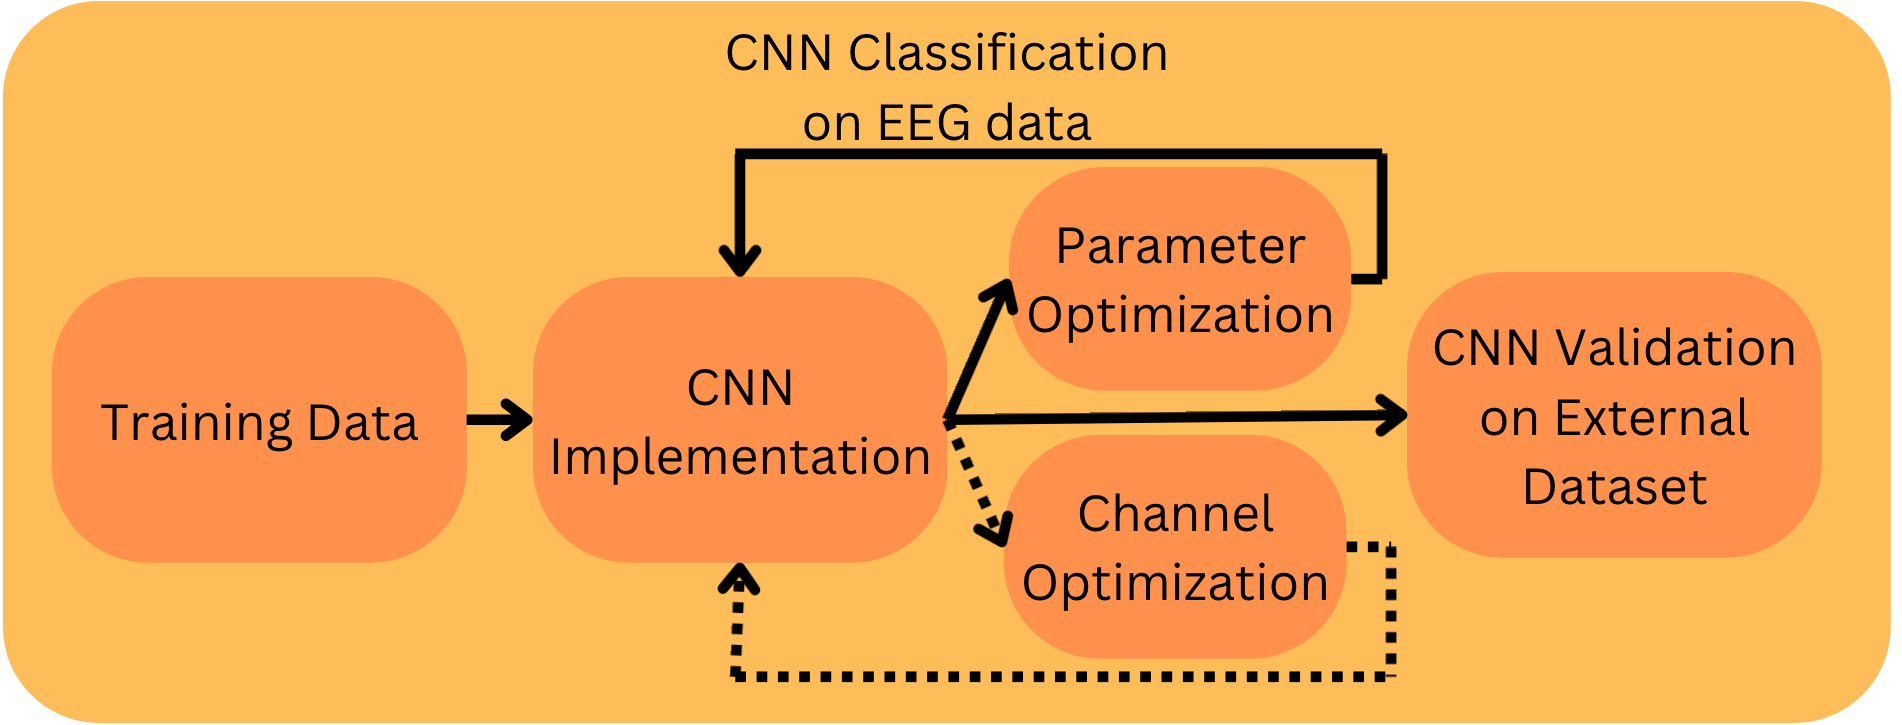
\includegraphics[width=400px]{Figures/cnn_flow.png}
    \caption{CNN Goal.}
    \label{fig:cnn_goal}
\end{figure}

\section{Scope of this Thesis}

This master's thesis builds upon the project initiated in Fall 2023 and is given in \autoref{Appendix C}. This research aims to develop and refine tools for objectively measuring contemplative practice proficiency using EEG data, focusing on crafting a robust machine-learning model. While the Project Thesis set out to collect measurements of novice meditators as they progressed, completing the Data Gathering step in \autoref{fig:overal_goal}, the primary contribution of this thesis is the development of a CNN based on the EEGNeX architecture, tailored to classify stages of contemplative proficiency and track progression over time. Hence, this thesis sets out to complete the CNN Implementation and Parameter Optimization steps in \autoref{fig:cnn_goal} and lay the groundwork for the objective data analysis step in \autoref{fig:overal_goal}. Training data collection, Channel Optimization, and CNN validation on external datasets from \autoref{fig:cnn_goal} are left for future work.

\subsection{Data Source and Model Training}
The project utilizes one of the publicly available EEG datasets, as described by \cite{Jin2019PredictingMW}. Their code can be found at \href{https://github.com/christina109/MW_EEG_CNN}{https://github.com/christina109/MW_EEG_CNN}, and the dataset can be found at \href{https://unishare.nl/index.php/s/T94LXPQqw5FEA4J}{https://unishare.nl/index.php/s/T94LXPQqw5FEA4J}. This dataset offers EEG recordings from participants engaged in tasks designed to induce and measure mind-wandering. The CNN model was trained to distinguish between 'on-task' and 'mind-wandering' states. The dataset has a dual-task framework involving both a Sustained Attention to Response Task (SART) and a Visual Search (VS) task, enabling the exploration of the classifier's task generality.

\subsection{Methodological Innovations}
Significant efforts were made to enhance the model's accuracy and generalizability:
Significant efforts were made to enhance the model's accuracy and generalizability:
\begin{itemize}
    \item \textbf{Individual and General Models}: Different CNN models were developed and tested, including personalized models for individual participants and a general model trained on the entire dataset with subsequent fine-tuning on personal data.
    \item \textbf{Data Balancing Techniques}: Various strategies were employed to address the imbalances inherent in the dataset, such as random undersampling, oversampling, and the Synthetic Minority Over-sampling Technique (SMOTE). Further innovation was introduced through the use of the Synthetic MEMD Minority Oversampling Technique (SMEMD-MOTE), specifically designed to handle the unique characteristics of EEG signals.
    \item \textbf{Noise and Artifact Reduction}: To improve data quality, unimportant Intrinsic Mode Functions (IMFs) were identified and removed, enhancing the signal clarity and, thereby, the reliability of the classification results.
\end{itemize}

\subsection{Evaluation and Results}
The effectiveness of these methodologies was rigorously tested through cross-validation within the dataset and by evaluating the model's ability to generalize across different individuals and tasks. Preliminary results indicate that the tailored CNN models, especially those undergoing individual-specific fine-tuning, show promising accuracy and task generality improvements. These models have potential applications in real-time monitoring and evaluation of mind-wandering states during various contemplative practices. While this is a promising first step, more research and data are necessary for a robust and trustworthy model.

\subsection{Aids}
Grammarly has been used in this report as a spellchecker and to rewrite sentences for clarity. Github Copilot has been used to autocomplete code and explain uncommented code by others.

The HPC system of NTNU has also been used to speed up the training of models throughout.
%\subsection{Stakeholders}

